\section{Introduction}
\textbf{Vocabulary:}
\begin{itemize}
    \item \textbf{Computer Vision:} all-embracing Notion
    \item \textbf{Machine Vision:} Emphasis on techniques for image aquisition, i.e. illumination, optics, camera techniques, real-time aspect, etc.
    \item \textbf{Image Processing:}Preprocessing, Segmentation, Object Detetction, Classification. AI, Machine Learning, Deep Learning: important techniques for e.g. classification tasks.
\end{itemize}

\subsection{Industrial Image Processing}
Very successful if restrictions regarding universality are made:
\begin{itemize}
    \item Precise description of the task
    \item All variations of samples (e.g. form, color, surface, etc.) and their variations (limiting samples) are available
    \item Ambient conditions will be adapted as necessary (illumination, handling) and are kept stable (ambient light, temperature, etc.)
\end{itemize}
Outside of these specifications the reliability of the system can not be guaranteed.

Superior to inspection by humans:
\begin{itemize}
    \item Fast
    \item Objective and stable results
    \item Automatic documentation possible
    \item Suited especially for production/inspection of mass-produced parts (e.g. 100\% inspection)
\end{itemize}
\begin{figure}[ht]
    \centering
    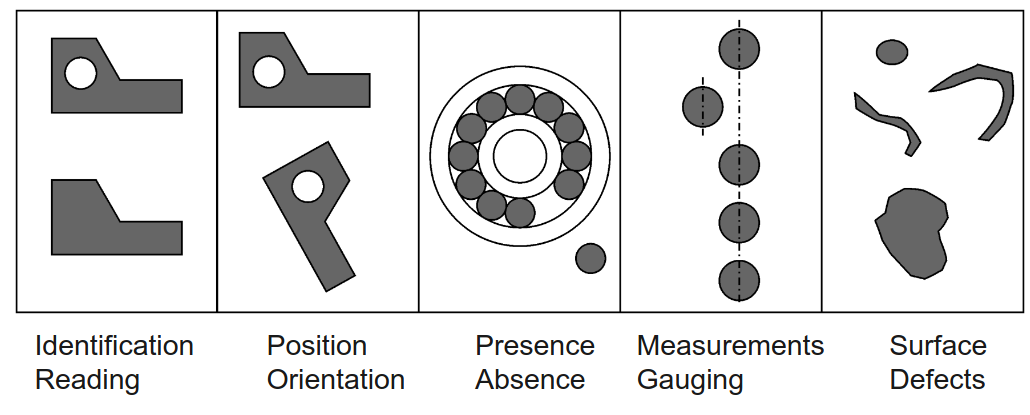
\includegraphics[width=0.8\columnwidth]{Images/01/IndustrialTasks.png}
    \caption{Typical Tasks of Industrial Image Processing}
    \label{fig:01_Introduction}
\end{figure}
